\documentclass[12pt]{report}
\usepackage{scribe,graphicx,graphics}
\usepackage{float}
\usepackage{siunitx}
\course{CSE 389D} 	
\coursetitle{Mathematical Modeling}	
\semester{Spring 2025}
\lecturer{} % Due Date: {\bf Mon, Oct 3 2016}}
\lecturetitle{Problem Set}
\lecturenumber{1}   
\lecturedate{}    
\usepackage{enumerate}
\newcommand{\remind}[1]{\textcolor{red}{\textbf{#1}}} %To remind me of unfinished work to fix later
\newcommand{\hide}[1]{} %To hide large blocks of code without using % symbols

\newcommand{\ep}{\varepsilon}
\newcommand{\vp}{\varphi}
\newcommand{\lam}{\lambda}
\newcommand{\Lam}{\Lambda}
%\newcommand{\abs}[1]{\ensuremath{\left\lvert#1\right\rvert}} % This clashes with the physics package
%\newcommand{\norm}[1]{\ensuremath{\left\lVert#1\right\rVert}} % This clashes with the physics package
\newcommand{\floor}[1]{\ensuremath{\left\lfloor#1\right\rfloor}}
\newcommand{\ceil}[1]{\ensuremath{\left\lceil#1\right\rceil}}
\newcommand{\A}{\mathbb{A}}
\newcommand{\B}{\mathbb{B}}
\newcommand{\C}{\mathbb{C}}
\newcommand{\D}{\mathbb{D}}
\newcommand{\E}{\mathbb{E}}
\newcommand{\F}{\mathbb{F}}
\newcommand{\K}{\mathbb{K}}
\newcommand{\N}{\mathbb{N}}
\newcommand{\Q}{\mathbb{Q}}
\newcommand{\R}{\mathbb{R}}
\newcommand{\T}{\mathbb{T}}
\newcommand{\X}{\mathbb{X}}
\newcommand{\Y}{\mathbb{Y}}
\newcommand{\Z}{\mathbb{Z}}
\newcommand{\As}{\mathcal{A}}
\newcommand{\Bs}{\mathcal{B}}
\newcommand{\Cs}{\mathcal{C}}
\newcommand{\Ds}{\mathcal{D}}
\newcommand{\Es}{\mathcal{E}}
\newcommand{\Fs}{\mathcal{F}}
\newcommand{\Gs}{\mathcal{G}}
\newcommand{\Hs}{\mathcal{H}}
\newcommand{\Is}{\mathcal{I}}
\newcommand{\Js}{\mathcal{J}}
\newcommand{\Ks}{\mathcal{K}}
\newcommand{\Ls}{\mathcal{L}}
\newcommand{\Ms}{\mathcal{M}}
\newcommand{\Ns}{\mathcal{N}}
\newcommand{\Os}{\mathcal{O}}
\newcommand{\Ps}{\mathcal{P}}
\newcommand{\Qs}{\mathcal{Q}}
\newcommand{\Rs}{\mathcal{R}}
\newcommand{\Ss}{\mathcal{S}}
\newcommand{\Ts}{\mathcal{T}}
\newcommand{\Us}{\mathcal{U}}
\newcommand{\Vs}{\mathcal{V}}
\newcommand{\Ws}{\mathcal{W}}
\newcommand{\Xs}{\mathcal{X}}
\newcommand{\Ys}{\mathcal{Y}}
\newcommand{\Zs}{\mathcal{Z}}
\newcommand{\ab}{\textbf{a}}
\newcommand{\bb}{\textbf{b}}
\newcommand{\cb}{\textbf{c}}
\newcommand{\db}{\textbf{d}}
\newcommand{\ub}{\textbf{u}}
\newcommand{\sbb}{\textbf{s}}
%\renewcommand{\vb}{\textbf{v}} % This clashes with the physics package (the physics package already defines the \vb command)
\newcommand{\wb}{\textbf{w}}
\newcommand{\xb}{\textbf{x}}
\newcommand{\yb}{\textbf{y}}
\newcommand{\zb}{\textbf{z}}
\newcommand{\vbb}{\textbf{v}}
\newcommand{\Ab}{\textbf{A}}
\newcommand{\Bb}{\textbf{B}}
\newcommand{\Cb}{\textbf{C}}
\newcommand{\Db}{\textbf{D}}
\newcommand{\eb}{\textbf{e}}
\newcommand{\ex}{\textbf{e}_x}
\newcommand{\ey}{\textbf{e}_y}
\newcommand{\ez}{\textbf{e}_z}
\newcommand{\zerob}{\mathbf{0}}
\newcommand{\abar}{\overline{a}}
\newcommand{\bbar}{\overline{b}}
\newcommand{\cbar}{\overline{c}}
\newcommand{\dbar}{\overline{d}}
\newcommand{\ubar}{\overline{u}}
\newcommand{\vbar}{\overline{v}}
\newcommand{\wbar}{\overline{w}}
\newcommand{\xbar}{\overline{x}}
\newcommand{\ybar}{\overline{y}}
\newcommand{\zbar}{\overline{z}}
\newcommand{\Abar}{\overline{A}}
\newcommand{\Bbar}{\overline{B}}
\newcommand{\Cbar}{\overline{C}}
\newcommand{\Dbar}{\overline{D}}
\newcommand{\Ubar}{\overline{U}}
\newcommand{\Vbar}{\overline{V}}
\newcommand{\Wbar}{\overline{W}}
\newcommand{\Xbar}{\overline{X}}
\newcommand{\Ybar}{\overline{Y}}
\newcommand{\Zbar}{\overline{Z}}
\newcommand{\Aint}{A^\circ}
\newcommand{\Bint}{B^\circ}
\newcommand{\limk}{\lim_{k\to\infty}}
\newcommand{\limm}{\lim_{m\to\infty}}
\newcommand{\limn}{\lim_{n\to\infty}}
\newcommand{\limx}[1][a]{\lim_{x\to#1}}
\newcommand{\liminfm}{\liminf_{m\to\infty}}
\newcommand{\limsupm}{\limsup_{m\to\infty}}
\newcommand{\liminfn}{\liminf_{n\to\infty}}
\newcommand{\limsupn}{\limsup_{n\to\infty}}
\newcommand{\sumkn}{\sum_{k=1}^n}
\newcommand{\sumk}[1][1]{\sum_{k=#1}^\infty}
\newcommand{\summ}[1][1]{\sum_{m=#1}^\infty}
\newcommand{\sumn}[1][1]{\sum_{n=#1}^\infty}
\newcommand{\emp}{\varnothing}
\newcommand{\exc}{\backslash}
\newcommand{\sub}{\subseteq}
\newcommand{\sups}{\supseteq}
\newcommand{\capp}{\bigcap}
\newcommand{\cupp}{\bigcup}
\newcommand{\kupp}{\bigsqcup}
\newcommand{\cappkn}{\bigcap_{k=1}^n}
\newcommand{\cuppkn}{\bigcup_{k=1}^n}
\newcommand{\kuppkn}{\bigsqcup_{k=1}^n}
\newcommand{\cappk}[1][1]{\bigcap_{k=#1}^\infty}
\newcommand{\cuppk}[1][1]{\bigcup_{k=#1}^\infty}
\newcommand{\cappm}[1][1]{\bigcap_{m=#1}^\infty}
\newcommand{\cuppm}[1][1]{\bigcup_{m=#1}^\infty}
\newcommand{\cappn}[1][1]{\bigcap_{n=#1}^\infty}
\newcommand{\cuppn}[1][1]{\bigcup_{n=#1}^\infty}
\newcommand{\kuppk}[1][1]{\bigsqcup_{k=#1}^\infty}
\newcommand{\kuppm}[1][1]{\bigsqcup_{m=#1}^\infty}
\newcommand{\kuppn}[1][1]{\bigsqcup_{n=#1}^\infty}
\newcommand{\cappa}{\bigcap_{\alpha\in I}}
\newcommand{\cuppa}{\bigcup_{\alpha\in I}}
\newcommand{\kuppa}{\bigsqcup_{\alpha\in I}}
\newcommand{\Rx}{\overline{\mathbb{R}}}
\newcommand{\dx}{\,dx}
\newcommand{\dy}{\,dy}
\newcommand{\dt}{\,dt}
\newcommand{\dax}{\,d\alpha(x)}
\newcommand{\dbx}{\,d\beta(x)}
\DeclareMathOperator{\glb}{\text{glb}}
\DeclareMathOperator{\lub}{\text{lub}}
\newcommand{\xh}{\widehat{x}}
\newcommand{\yh}{\widehat{y}}
\newcommand{\zh}{\widehat{z}}
\newcommand{\<}{\langle}
\renewcommand{\>}{\rangle}
\renewcommand{\iff}{\Leftrightarrow}
\DeclareMathOperator{\im}{\text{im}}
\let\spn\relax\let\Re\relax\let\Im\relax
\DeclareMathOperator{\spn}{\text{span}}
\DeclareMathOperator{\sym}{\text{Sym}}
\DeclareMathOperator{\myskew}{\text{Skew}}
\DeclareMathOperator{\Re}{\text{Re}}
\DeclareMathOperator{\Im}{\text{Im}}
\DeclareMathOperator{\diag}{\text{diag}}
\endinput

\theoremheaderfont{\itshape}
\theorembodyfont{\upshape}
\newtheorem{case}{Case}

% Insert your name here!
\scribe{Student Name: Noah Reef}
\newcommand{\rb}{\bold{r}}

\begin{document}
\maketitle

\section*{Problem 1}
\subsection*{Part a}
\begin{equation*}
    L(\rb,\dot{\rb},t) = \frac{1}{2}m\dot{\rb}^2
\end{equation*}
\subsection*{Part b}
Using Euler-Lagrange equation, we have:
\begin{equation*}
    \frac{\partial L}{\partial \rb} - \frac{d}{dt}\left(\frac{\partial L}{\partial \dot{\rb}}\right) =  -m\ddot{\rb} = 0
\end{equation*}
this gives us the general solution
\begin{equation*}
    \rb(t) = c_2 t + c_1
\end{equation*}
using the boundary conditions, $\rb(t_1) = \rb_1$ and $\rb(t_2) = \rb_2$ with $t_2 < t_1$ we get that
\begin{align*}
    \rb(t_1) &= \bold{c}_2t_1 + \bold{c}_1 = \rb_1 &\implies \bold{c}_1 = \rb_1 - \bold{c}_2t_1 \\
    \rb(t_2) &= \bold{c}_2 t_2 + (\rb_1 - \bold{c}_2t_1) = \rb_2 &\implies \bold{c_2} = \frac{\rb_2 - \rb_1}{(t_2 - t_1)}
\end{align*}
thus the particular solution is
\begin{equation*}
    \rb(t) = \left(\frac{\rb_2 - \rb_1}{t_2-t_1}\right)(t-t_1) + \rb_1
\end{equation*}
\subsection*{Part c}
Recall that the action is given by
\begin{align*}
    S[\rb_1,\rb_2; \rb(t)] &= \int_{t_1}^{t_2} L \, dt \\
                           &= \frac{m}{2}\left[\si{kg}\right]\int_{t_1}^{t_2} \dot{\rb}^2 \left[\si{m^2\per s^2}\right] \, dt \\
                           &= \frac{m}{2}\left[\si{kg}\right] \int_{t_1}^{t_2} \left(\frac{\rb_2 - \rb_1}{t_2 - t_1}\right)^2 \left[\si{m^2\per s^2}\right] \, dt \\
                           &= \frac{m}{2}\left[\si{kg}\right]  \left(\frac{\rb_2 - \rb_1}{t_2 - t_1}\right)^2 (t_2 - t_1) \left[\si{m^2\per s}\right]\\
                           &= \frac{m}{2}\frac{(\rb_2 - \rb_1)^2}{t_2 - t_1}\left[\si{kg \cdot m^2\per s}\right]\\
                           &= \frac{m}{2}\frac{(\rb_2 - \rb_1)^2}{t_2 - t_1}\left[\si{J \cdot s}\right]
\end{align*}

\subsection*{Part d}
\begin{align*}
    S_{\text{electron}} &= \frac{9.11 \times 10^{-31}}{2}\frac{(1 \times 10^{-9} \si{m})^2}{1 \times 10^{-9}\si{s}} = 4.55 \times 10^{-40} = 4.31\times 10^{-6} \hbar \\
    S_{\text{Earth}} &= \frac{5.97 \times 10^{24} }{2}\frac{(1 \times 10^{-9} \si{m})^2}{1 \times 10^{-9}\si{s}} = 2.985 \times 10^{15} = 2.829 \times 10^{49} \hbar
\end{align*}

\subsection*{Part e}
Considering the family of trajectories given by
\begin{equation*}
    \rb_\lambda(t) = \rb_0(t) + \lambda \bold{c} \sin\left[\pi \frac{t-t_1}{t_2 - t_1}\right]
\end{equation*}
we compute the actions as
\begin{align*}
    S &= \frac{m}{2} \int_{t_1}^{t_2} \dot{\rb_\lambda}^2 \, dt \\
      &= \frac{m}{2} \int_{t_1}^{t_2} \dot{\rb}_0(t)^2 + 2 \left(\frac{\pi \lambda}{t_2 -t_1}\right)\bold{c} \cdot \dot{\rb}_0(t) \cos\left(\pi \frac{t - t_1}{t_2 - t_1}\right) + \left(\frac{\pi \lambda \bold{c}}{t_2 -t_1}\right)^2 \cos^2\left(\pi \frac{t - t_1}{t_2 - t_1}\right) \\
      &=  \frac{m}{2}\frac{(\rb_2 - \rb_1)^2}{t_2 - t_1} + 0 + \frac{m(\pi \lambda \bold{c})^2}{4(t_2-t_1)} \\
      &= \frac{2m(\rb_2 - \rb_1)^2 + m(\pi\lambda \bold{c})^2}{4(t_2-t_1)}
\end{align*}

\subsection*{Part f}
We consider the slightly perturbed trajectory from $\rb_0(t)$ by $\delta \lambda$, then we can clearly see that as $\delta \lambda \to 0$, then we have that
\begin{equation*}
    \lim_{\delta \lambda \to 0} \frac{m}{2}\frac{(\rb_2 - \rb_1)^2}{t_2 - t_1} + \frac{m(\pi \delta\lambda \bold{c})^2}{4(t_2-t_1)} = \frac{m}{2}\frac{(\rb_2 - \rb_1)^2}{t_2 - t_1} = S
\end{equation*}
which implies that $\delta S = 0$.

\section*{Problem 2}
\subsection*{Part a}
\begin{equation*}
  L(x, \dot{x}, t) = T - V = \frac{1}{2}m\dot{x}^2 - \frac{1}{2}kx^2
\end{equation*}
\subsection*{Part b}
Using the Euler-Lagrange equation, we have:
\begin{equation*}
  \frac{\partial L}{\partial x} - \frac{d}{dt}\left(\frac{\partial L}{\partial \dot{x}}\right) = -kx - m \ddot{x} = 0
\end{equation*}
solving the differential equation above gives the general solution,
\begin{equation*}
  x(t) = c_2 \sin\left(\omega t\right) + c_1 \cos\left(\omega t\right)
\end{equation*}
where $\omega = \sqrt{\frac{k}{m}}$. Then we see with boundary equations that
\begin{align*}
  x(0) &= c_1 = x_1 \\
  x(\tau) &= c_2 \sin\left(\omega \tau\right) + x_1 \cos\left(\omega \tau\right) = x_2
\end{align*}
solving for $c_2$ gives
\begin{equation*}
  c_2 = \frac{x_2 - x_1 \cos\left(\omega \tau\right)}{\sin\left(\omega \tau\right)}
\end{equation*}
since $\tau \neq \frac{n\pi}{\omega}$, we have that $\sin(\omega \tau) \neq 0$. 

\subsection*{Part c}
To solve for the action $S$, we have that
\begin{align*}
  S &= \int_0^\tau L(x, \dot{x}, t) dt \\
    &= \int_0^\tau \left(\frac{1}{2}m\dot{x}^2 - \frac{1}{2}kx^2\right) dt \\
    &= \frac{1}{2}m\int_0^\tau \dot{x}^2 - \omega^2 x^2 \, dt \\ 
\end{align*}
Now notice that
\begin{align*}
  \int_0^\tau \dot{x}^2 \, dt &= x\dot{x}\Big|_0^\tau - \int_0^\tau x\ddot{x} \, dt 
\end{align*}
and since $\ddot{x} = -\omega^2 x$, we have that
\begin{equation*}
  \int_0^\tau \dot{x}^2 \, dt = x\dot{x}\Big|_0^\tau + \omega^2 \int_0^\tau x^2 \, dt
\end{equation*}
Thus, we have that
\begin{equation*}
  S = \frac{1}{2}m\left(x\dot{x}\Big|_0^\tau + \omega^2 \int_0^\tau x^2 \, dt - \omega^2 \int_0^\tau x^2 \, dt \right)
\end{equation*}
thus
\begin{equation*}
  S = \frac{1}{2}m\left(x\dot{x}\Big|_0^\tau\right)
\end{equation*}
to solve the inside term we have that
\begin{align*}
  x\dot{x} &= \left(c_2 \sin(\omega t) + x_1 \cos(\omega t)\right) (\omega c_2 \cos(\omega t) - x_1 \omega \sin(\omega t)) 
\end{align*}
now evaluating at $\tau$ and $0$ gives
\begin{align*}
  x\dot{x}\Big|_0^\tau &= \left(c_2 \sin(\omega \tau) + x_1 \cos(\omega \tau)\right) (\omega c_2 \cos(\omega \tau) - x_1 \omega \sin(\omega \tau))-  x_1\omega c_2 \\
                       &= \left(\frac{x_2 - x_1\cos(\omega \tau)}{\sin(\omega \tau)} \sin(\omega \tau) + x_1\cos(\omega \tau)\right) \left(\frac{\omega x_2\cos(\omega \tau)-\omega x_1 \cos^2(\omega \tau)}{\sin(\omega \tau)} - x_1 \omega \sin(\omega \tau)\right) - \dots \\
                       &= \frac{\omega x_2^2 \cos(\omega \tau) - \omega x_2x_1}{\sin(\omega \tau)} - \frac{\omega x_1x_2 - \omega x_1^2 \cos(\omega \tau)}{\sin(\omega \tau)} \\
                       &= \frac{\omega}{\sin(\omega \tau)}(-2x_1x_2 + (x_1^2 + x_2^2)\cos(\omega \tau))
\end{align*}
thus 
\begin{equation*}
  S = \frac{m\omega}{2\sin(\omega \tau)}(-2x_1x_2 + (x_1^2 + x_2^2)\cos(\omega \tau))
\end{equation*}

\subsection*{Part d}
To write the action $S(x,\tau)$, we set $x_2 = x$ and $x_1 = 0$ to get 
\begin{equation*}
  S(x,\tau) = \frac{m\omega}{2\sin(\omega \tau)}( x^2\cos(\omega \tau))
\end{equation*}
to solve for the action of a silicon atom, with mass $m_{\text{Si}} = 4.66 \times 10^{-26} \si{kg}$, vibrating at frequecy $\omega = 15\si{THz}$ and amplitude $x = a_0$ and a time $\tau = \pi/(4\omega)$
\begin{align*}
    S(x,\tau) &= \frac{(4.66 \times 10^{-26})(15\times 10^{12})}{2\sin(\pi/4)} ((5.29 \times 10^{-11})^2 \cos(\pi/4)) \\
    &= 9.78 \times 10^{-34} \\
    &= 9.27 \hbar
\end{align*}

\section*{Problem 3}
\subsection*{Part a}
\begin{equation*}
    L(\rb_1,\rb_2, \dot{\rb}_1, \dot{\rb}_2,t) = \frac{1}{2}(m_1\dot{\rb}_1^2 + m_2\dot{\rb}_2^2) - G\frac{m_1m_2}{|\rb_1 -\rb_2|}
\end{equation*}
\subsection*{Part b}
Define
\begin{equation*}
    \bold{R} = \frac{m_1\rb_1 + m_2\rb_2}{m_1 + m_2} \quad \text{ and } \quad \rb = \rb_2 - \rb_1
\end{equation*}
then we get that 
\begin{align*}
    \dot{\bold{R}}^2 = \frac{m_1^2 \dot{\rb}_1^2 + 2m_1m_2\dot{\rb}_1\dot{\rb}_2 + m_2^2 \dot{\rb}_2^2}{(m_1 + m_2)^2} \quad \text{ and } \quad \dot{\rb}^2 = \dot{\rb}_2^2 - 2\dot{\rb}_1 \dot{\rb}_2 + \dot{\rb}_1^2
\end{align*}
then by setting 
\begin{align*}
    M &= m_1 + m_2 \\
    \mu &= \frac{m_1m_2}{m_1 + m_2} = \frac{m_1m_2}{M} \\
    k &= -Gm_1m_2
\end{align*}
clearly we get that
\begin{equation*}
    -G\frac{m_1m_2}{|\rb_1 - \rb_2|} = \frac{k}{|\rb|}
\end{equation*}
additionally we see that,
\begin{align*}
 \frac{1}{2}(M\dot{\bold{R}}^2 + \mu \dot{\rb}^2) &= \frac{1}{2M} \left(m_1^2 \dot{\rb}_1^2 + 2m_1m_2\dot{\rb}_1\dot{\rb}_2 + m_2^2 \dot{\rb}_2^2 + m_1m_2\dot{\rb}_2^2 - 2m_1m_2\dot{\rb}_1 \dot{\rb}_2 + m_1m_2\dot{\rb}_1^2\right) \\
 &= \frac{1}{2M} (m_1\dot{\rb}_1^2(m_1 + m_2) + m_2\dot{\rb}_2^2(m_1 + m_2)) \\
 &= \frac{1}{2M} (m_1\dot{\rb}_1^2M + m_2\dot{\rb}_2^2M) \\
 &= \frac{1}{2}(m_1\dot{\rb}_1^2 + m_2\dot{\rb}_2^2)
\end{align*}
thus 
\begin{equation*}
    L = \frac{1}{2}(m_1\dot{\rb}_1^2 + m_2\dot{\rb}_2^2) - G\frac{m_1m_2}{|\rb_1 -\rb_2|} =  \frac{1}{2}(M\dot{\bold{R}}^2 + \mu \dot{\rb}^2) + \frac{k}{|\rb|}
\end{equation*}

\subsection*{Part c}
For the Euler-Lagrange Equations in this reference frame we get that
\begin{equation*}
   \begin{cases} \frac{\partial L}{\partial \bold{R}} - \frac{d}{dt}\left(\frac{\partial L}{\partial \dot{\bold{R}}}\right) = M\ddot{\bold{R}} = 0 \\
   \frac{\partial L}{\partial \rb} - \frac{d}{dt}\left(\frac{\partial L}{\partial \dot{\rb}}\right)  = 0 
   \end{cases}
\end{equation*}
solving the above differential equations give,
\begin{align*}
    M\ddot{\bold{R}} &= 0 \implies \bold{R} = c_2t + c_1 \\
\end{align*}
thus the center of mass $R$ has rectilinear motion.

\subsection*{Part d}
Recall that the angular momentum is given by
\begin{equation*}
    \bold{L} = \frac{1}{2}\mu \dot{\rb}^2 + \frac{k}{|\rb|}
\end{equation*}
taking the derivative with respect to time yields
\begin{equation*}
    \frac{\partial \bold{L}}{\partial t} = \dot{\rb} \times \mu \dot{\rb} + \rb \times \mu \ddot{\rb} = \rb \times \mu \ddot{\rb}
\end{equation*}
then from the Euler-Lagrangian equation above we have that
\begin{equation*}
    \mu \ddot{r} = -\frac{k}{|\rb|^3}\rb
\end{equation*}
and thus 
\begin{equation*}
     \frac{\partial \bold{L}}{\partial t} = \rb \times \mu \ddot{\rb} = \rb \times -\frac{k}{|\rb|^3}\rb = 0
\end{equation*}
thus the angular momentum is a constant of motion.

\subsection*{Part e}
let 
\begin{equation*}
    \rb = \begin{bmatrix}
        x(t)  \\ y(t) \\ 0
    \end{bmatrix} = \begin{bmatrix}
        r(t)\cos(\theta(t)) \\ r(t)\sin(\theta(t)) \\ 0
    \end{bmatrix}
\end{equation*}
then we see that
\begin{align*}
    \dot{\rb} &= \begin{bmatrix}
        \dot{r}\cos(\theta) - r\dot{\theta} \sin(\theta) \\
        \dot{r}\sin(\theta) + r\dot{\theta} \cos(\theta) \\
        0
    \end{bmatrix} \implies \dot{\rb}^2 = \dot{r}^2  +r^2\dot{\theta}^2 \\
    |\rb| &= \sqrt{r^2\cos^2(\theta) + r^2\sin^2(\theta) + 0 } = r
\end{align*}
and hence
\begin{equation*}
    L = \frac{1}{2}\mu \dot{\rb}^2 + \frac{k}{|\rb|} = \frac{1}{2}\mu (\dot{r}^2 + r^2\dot{\theta}^2) + \frac{k}{r}
\end{equation*}
\subsection*{Part f}
Taking 
\begin{equation*}
    \bold{L} = \rb \times \mu \dot{\rb} = \det\left(\begin{bmatrix}
        \hat{x} & \hat{y} & \hat{z} \\
        r\cos(\theta) & r\sin(\theta) & 0 \\
        \mu \dot{r}\cos(\theta) - \mu\dot{\theta} \sin(\theta) & \mu\dot{r}\sin(\theta) + \mu r \dot{\theta} \cos(\theta) & 0
    \end{bmatrix}\right) = \mu r^2 \dot{\theta}
\end{equation*}
\subsection*{Part g}
\begin{equation*}
    \begin{cases}
        \frac{\partial L}{\partial r} - \frac{d}{dt}\left(\frac{\partial L}{\partial \dot{r}}\right) &= \mu r \dot{\theta}^2 - \frac{k}{r^2} - \mu \ddot{r} = 0 \\
        \frac{\partial L}{\partial \theta} - \frac{d}{dt}\left(\frac{\partial L}{\partial \dot{\theta}}\right) &=\frac{d}{dt}(\mu r^2 \dot{\theta}) = 0 \\
    \end{cases}
\end{equation*}
\subsection*{Part h}
Recall that
\begin{equation*}
    l = \mu r^2 \dot{\theta} \implies \dot{\theta} = \frac{l}{\mu r^2}
\end{equation*}
thus replacing it into the top Euler-Lagrange equation yields,
\begin{equation*}
    \mu r \left(\frac{l}{\mu r^2}\right)^2 = \frac{k}{r^2} + \mu \ddot{r}
\end{equation*}
and gives the Lagrangian as
\begin{equation*}
    L(r,\dot{r}) = \frac{1}{2}\mu \left(\dot{r}^2 + \frac{l^2}{\mu^2r^2}\right) + \frac{k}{r}
\end{equation*}

\subsection*{Part i}
We compute the conjugate momentum as
\begin{equation*}
    p =\frac{\partial L}{\partial \dot{r}} = \mu \dot{r}
\end{equation*}
which gives us the Hamiltonian as
\begin{align*}
    H &= p\dot{r} - L(r,\dot{r}) = (\mu \dot{r})\dot{r} - \left(\frac{1}{2}\mu \dot{r}^2 + \frac{k}{r} - \frac{l^2}{2\mu r^2}\right) \\
    &= \frac{1}{2}\mu \dot{r}^2 - \frac{k}{r} + \frac{l^2}{2\mu r^2} \tag{$\dot{r} = p/\mu$}\\
    &= \frac{p^2}{2\mu} - \frac{k}{r} + \frac{l^2}{2\mu r^2}
\end{align*}
\subsection*{Part j}
Compute the Hamiltonian equations as
\begin{equation*}
\begin{cases}
\dot{r} &= \frac{\partial H}{\partial p} = \frac{p}{\mu} \\
\dot{p} &=-\frac{\partial H}{\partial r} = -\frac{k}{r^2} + \frac{l^2}{\mu r^3}
\end{cases}    
\end{equation*}
and see that
\begin{equation*}
    E = T + V = \frac{p^2}{2\mu} - \frac{k}{r} + \frac{l^2}{2\mu r^2}
\end{equation*}
then we have that
\begin{equation*}
    \dot{E} = \frac{\partial E}{\partial r}\dot{r} + \frac{\partial E}{\partial p} \dot{p} = -\dot{p}\dot{r} + \frac{p}{\mu} \dot{p} = -\dot{p}\dot{r} + \dot{r}\dot{p} = 0
\end{equation*}
thus the total energy is a constant of time.

\subsection*{Part k}
Let $x = r/r_0$, then we have that $r = xr_0$ and 
\begin{align*}
    V(r) = -\frac{k}{xr_0} + \frac{l^2}{2\mu (r_0x)^2} &= -\frac{2E_0}{x} + \frac{1}{kr_0}E_0 \frac{l^2}{\mu x^2} \\
    &= -\frac{2E_0}{x} + \frac{E_0}{x^2}
\end{align*}
then the plot is
\begin{equation*}
    V(r)/E_0 = -\frac{2}{x} + \frac{1}{x^2}
\end{equation*}

\begin{figure}[H]
    \centering
    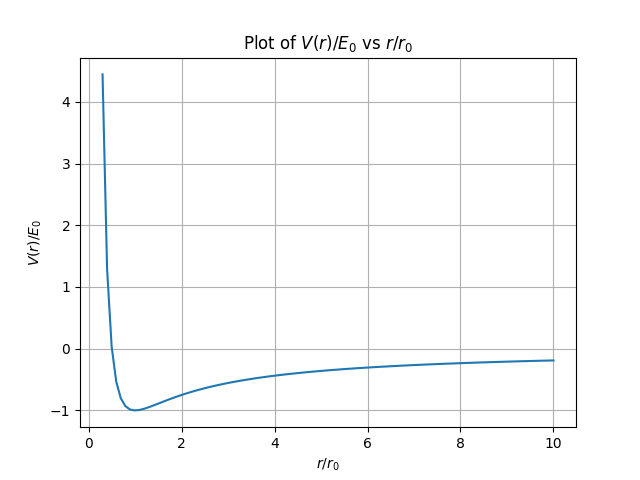
\includegraphics[scale=0.7]{CSE_389D/ps_1/Q3_Pk.png}
    \caption{Plot of $V/E_0$ vs $r/r_0$}
    \label{fig:enter-label}
\end{figure}

\subsection*{Part l}
\begin{case}[$E = -E_0$]
    If $E = -E_0$, then we have that
    \begin{equation*}
        E = T + V \implies T = E - V = -E_0 - V
    \end{equation*}
    note that since $T \geq 0$, looking at the graph we then require $V = -E_0$ hence $T = 0$ with constant radius $r = r_0$. 
\end{case}
\begin{case}[$-E_0 < E < 0$]
    If $-E_0 < E < 0$, then we have that
    \begin{equation*}
     -E_0 - V < T < -V
    \end{equation*}
\end{case}
which gives us an ellipse.

\begin{case}[$E \geq 0$]
    Then here we can see that $T  = E - V$ grows without bound past $r = r_0$ and hence is a hyperbolic trajectory.
\end{case}

\subsection*{Part m}
Recall that 
\begin{equation*}
    V(r) = -\frac{k}{r} + \frac{l^2}{2\mu r^2} 
\end{equation*}
whose second-order Taylor Expansion is given by
\begin{equation*}
    V(r) \approx V(r_0) + V'(r_0) (r-r_0) + \frac{1}{2} V''(r_0)(r-r_0)^2 = -E_0 + \frac{1}{2}V''(r_0)(r-r_0)^2
\end{equation*}
plugging back into the Lagrangian yields
\begin{equation*}
    L = \frac{1}{2}\mu \dot{r}^2 - \frac{1}{2}V''(r_0)(r-r_0)^2 + E_0
\end{equation*}
computing the Euler-Lagrange equation yields
\begin{equation*}
    \mu \ddot{r} = -V''(r_0)(r-r_0)
\end{equation*}
this then gives us
\begin{equation*}
    r(t) = c_2 \sin\left(\omega t\right) + c_1\cos(\omega t) + r_0
\end{equation*}
where $\omega = \sqrt{(V''(r_0)r_0)/\mu}$. Using intitial conditions we get that
\begin{equation*}
    r(t) = r_0 + \frac{r_\text{max} - r_{\text{min}}}{2}\cos(\omega t)
\end{equation*}

\subsection*{Part n}
Recall that
\begin{equation*}
    \dot{\theta} = \frac{l}{\mu r^2} \approx \frac{l}{\mu r_0^2}
\end{equation*}
and thus $\theta(t) \approx \frac{l}{(\mu r_0^2)}t + \theta_0$

\subsection*{Part o}
From n we get that
\begin{equation*}
    t \approx \frac{\mu r_0^2}{l}(\theta - \theta_0)
\end{equation*}
and hence
\begin{equation*}
    r(\theta) \approx r_0 + \frac{r_\text{max} - r_{\text{min}}}{2}\cos\left(\omega\frac{\mu r_0^2}{l}(\theta - \theta_0) \right)
\end{equation*}
which represents an ellipse in the $xy$-plane.

\subsubsection*{Part p}
Let 
\begin{align*}
    m_{\text{Earth}} &= 5.97 \times 10^{24} \si{kg} \\
    m_{\text{Sun}} &= 1.99 \times 10^{30} \si{kg} \\
    G &= 6.67 \times 10^{-11} \si{m^3 kg^{-1} s^{-1}}
\end{align*}
recall that
\begin{equation*}
    \mu = \frac{m_1m_2}{m_1 + m_2} \quad \text{and} \quad k = -Gm_1m_2
\end{equation*}
and assume that $\dot{\theta} = \frac{2\pi}{365 \text{ days}} = \frac{2\pi}{3.154 \times 10^7s}$
\begin{equation*}
    r_0 = l^2/(\mu k) = \frac{(\mu r_0^2 \dot{\theta})^2}{\mu k}
\end{equation*}
solving the above gives us $r_0 \approx 1.4955 \times 10^{11}\si{m} $ which is close to the expected measured distance of $1.495978707 \times 10^{11} \si{m}$
\section*{Problem 4}
\subsection*{Part a}
Recall that the conjugate momentum is computed as
\begin{equation*}
    \bold{p} = \frac{\partial L}{\partial \dot{\rb}} = m \dot{\rb} + qA
\end{equation*}

\subsection*{Part b}
Recall that the Hamiltonian is computed by
\begin{align*}
    H &= \dot{p}\dot{\rb} - L \\
      &= (m\dot{\rb}+ qA) \dot{\rb}  - \frac{1}{2}m \dot{\rb}^2 + q\varphi - q\dot{\rb} \cdot A \\
      &= \frac{1}{2} m\dot{\rb}^2 + q\varphi \\
\end{align*}
note that
\begin{equation*}
    \dot{\rb} = \frac{(\bold{p}-qA)}{m}
\end{equation*}
so we get that
\begin{equation*}
    H = \frac{(\bold{p} - qA)^2}{2m} + q\varphi
\end{equation*}
\subsection*{Part c}
Recall that the Hamiltonian Equations are found as
\begin{equation*}
    \begin{cases}
        \dot{\rb} &= \phantom{-} \frac{\partial H}{\partial \bold{p}} \\
        \dot{\bold{p}} &= - \frac{\partial H}{\partial \rb}
    \end{cases}
\end{equation*}
and get that
\begin{equation*}
    \dot{\rb} = \frac{\partial H}{\partial \bold{p}} = \frac{(\bold{p} - qA)}{m}
\end{equation*}
and
\begin{align*}
    \dot{\bold{p}} =  -\frac{\partial H}{\partial \rb} = -\frac{1}{2m} \nabla^{\rb}\left(\bold{p} - qA\right)^2 - q \nabla^{\rb}\varphi 
\end{align*}
then we see that 
\begin{equation*}
    \nabla^{\rb}\left(\bold{p} - qA\right)^2 = 2 (\bold{p} - qA) \cdot \nabla^{\rb})(\bold{p} - qA) + 2(\bold{p} - qA) \times (\nabla^{\rb} \times (\bold{p} - qA))
\end{equation*}
note that
\begin{align*}
    \nabla^{\rb} \times (\bold{p} - qA) &= (\nabla^{\rb} \times \bold{p}) - q(\nabla^{\rb} \times A) = -qB \\
\end{align*}
and so we get that
\begin{align*}
     \nabla^{\rb} (\bold{p} - qA)^2 &=-2q(\bold{p} - qA)\cdot (\nabla^{\rb}A) - 2q\left[(\bold{p} - qA) \times B\right]
\end{align*}
then we replace $\bold{p} - qA = m\dot{\rb}$ to get
\begin{equation*}
    \nabla^{\rb} (\bold{p} - qA)^2 =-2q(m\dot{\rb})\cdot (\nabla^{\rb}A) - 2qm\left[\dot{\rb} \times B\right]
\end{equation*}
and hence
\begin{equation*}
    \dot{\bold{p}} = q(\dot{\rb} \cdot \nabla^{\rb})A + q(\dot{\rb} \times B) - q\nabla^{\rb}\varphi
\end{equation*}

\subsection*{Part d}
Now by taking the second derivative of position
\begin{align*}
    m\ddot{\rb} = \frac{d}{dt}(\bold{p} - qA) &= \dot{\bold{p}} - q\left(\nabla^{\rb}A \cdot \dot{\rb} + \frac{\partial A}{\partial t}\right) \\
    &= \left[q(\dot{\rb} \cdot \nabla^{\rb})A + q(\dot{\rb} \times B) - q\nabla^{\rb}\varphi\right] - q\left(\nabla^{\rb}A \cdot \dot{\rb} + \frac{\partial A}{\partial t}\right) \\
    &= q(\dot{\rb} \times B) + qE = q(E + \dot{\rb} \times B)
\end{align*}
\subsection*{Part e}
Suppose that the vector field $A$ was defined by
\begin{equation*}
    A = \frac{B}{2}(x \bold{u}_y - y\bold{u}_x) = \begin{bmatrix}
        -(1/2)By \\ \phantom{-}(1/2)Bx \\
        0
    \end{bmatrix}
\end{equation*}
then we compute $B$ as
\begin{equation*}
    B = \nabla \times A = \left(\frac{\partial A_z}{\partial y} - \frac{\partial A_y}{\partial z}\right)\bold{u}_x + \left(\frac{\partial A_x}{\partial z} - \frac{\partial A_z}{\partial x}\right)\bold{u}_y + \left(\frac{\partial A_y}{\partial x} - \frac{\partial A_x}{\partial y}\right)\bold{u}_z
\end{equation*}
note that since $A$ has no $z$ component term we are left with
\begin{equation*}
    B = \left(\frac{\partial A_y}{\partial x} - \frac{\partial A_x}{\partial y}\right)\bold{u}_z = \frac{B}{2} - \left(-\frac{B}{2}\right) \bold{u}_z = B \bold{u}_z
\end{equation*}

\subsection*{Part f}
Using the magnetic field of (e) and setting the scalar potential to $\varphi = 0$ yields
\begin{equation*}
    H = \frac{(\bold{p} - qA)^2}{2m}
\end{equation*}
note that
\begin{equation*}
    (\bold{p} - qA)^2 = \bold{p^2} - 2q\bold{p} \cdot A + q^2 A^2
\end{equation*}
additonally we see that
\begin{equation*}
    \bold{p} \cdot A = \frac{B}{2}\left(-y \bold{p}_x +x \bold{p}_y\right)
\end{equation*}
which we see that
\begin{equation*}
    \rb \times \bold{p} = \bold{u}_x(yp_z - zp_y) - \bold{u}_y(xp_z - zp_x) + \bold{u}_z(xp_y - yp_x)
\end{equation*}
and hence 
\begin{equation*}
    (\bold{r} \times \bold{p}) \cdot B = B(xp_y - yp_x)
\end{equation*}
thus 
\begin{equation*}
    \bold{p} \cdot A = \frac{1}{2}(\bold{r} \times \bold{p}) \cdot B = \frac{1}{2} \bold{L} \cdot B
\end{equation*}
and hence that Hamiltonian is
\begin{equation*}
    H = \frac{\bold{p}^2}{2m} - \frac{q}{2m} \bold{L} \cdot B + q^2 A^2
\end{equation*}
\section*{Problem 5}
\subsection*{Part a}
\begin{align*}
    \frac{|\nabla S(\rb,t)|^2}{2m} + V(\rb) = -\frac{\partial S(\rb,t)}{\partial t}
\end{align*}
this gives
\begin{equation*}
    \frac{1}{2m}(x^2m^2\omega^2 \cot^2(\omega \tau)) + \frac{1}{2}(m\omega^2)x^2 = \frac{1}{2}m\omega^2x^2 \csc^2(\omega \tau)
\end{equation*}
which can be rewritten as
\begin{equation*}
    \frac{2}{mx^2} S^2 +  \frac{1}{2}m\omega^2 x^2 = \frac{1}{2}m\omega^2 x^2 + \frac{2S^2}{mx^2}
\end{equation*}
or
\begin{equation*}
     \frac{2}{mx^2} S^2 = \frac{2S^2}{mx^2}
\end{equation*}

\subsection*{Part b}
See that if we plug-in $S = 9.27 \hbar$
we get
\begin{equation*}
    \frac{2}{mx^2} (9.27 \hbar)^2 = \frac{2}{mx^2} (9.27 \hbar)^2
\end{equation*}
which obviously agrees.

\subsection*{Part c}
Recall that for a free particle $V(\rb) = 0$, thus we have that
\begin{equation*}
   \frac{1}{2m}|\nabla S(x,y,z,t)|^2 = -\frac{\partial S(x,y,z,t)}{\partial t}
\end{equation*}

\subsection*{Part d}
\begin{equation*}
    S(x,y,z,t) = X(x) + Y(y) + Z(z) + T(t)
\end{equation*}
which then plugging into the Hamilton-Jacobi Equation yields
\begin{equation*}
    \frac{1}{2m}\left[\left(\frac{\partial X(x)}{\partial x}\right)^2 + \left(\frac{\partial Y(y)}{\partial y}\right)^2 + \left(\frac{\partial Z(z)}{\partial z}\right)^2\right] = - \frac{dT}{dt} = E 
\end{equation*}
and we take the spatial derivatives to be constants, yielding
\begin{equation*}
    \frac{\partial X}{\partial x} = p_x \quad \frac{\partial Y}{\partial y} = p_y \quad \frac{\partial Z}{\partial z} = p_z 
\end{equation*}
which gives us
\begin{equation*}
    X(x) = xp_x \quad Y(y) = yp_y \quad Z(z) = zp_z
\end{equation*}
and
\begin{equation*}
    E = \frac{1}{2m}(p_x^2 + p_y^2 + p_z^2) = \frac{1}{2m}\bold{p}^2
\end{equation*}
which gives us that
\begin{equation*}
    T(t) = -\frac{1}{2m}\bold{p}^2 t
\end{equation*}
which gives us the final expression for $S$ as
\begin{equation*}
    S(x,y,z,t) = \bold{p} \cdot \bold{r} - \frac{1}{2m} \bold{p}^2 t
\end{equation*}
\end{document}
